\section{Simulated mutli-channel signal}
\label{sc:mysimulation}
To demonstrate the signal processing approach, this section generates simulated signals at high resolution, ranging from 40cm down to 10cm. As mentioned, as the resolution decreases (i.e. improves) data capture and storage requirements rapidly increase which also means that hardware requirements for signal processing also increase. The highest resolution of 10cm, simulated in this section, required a significant amount of processing power, time and Random Access Memory (RAM). Simulations mode was produced by using the Vienna Supercomputing Cluster (VSC) for which the authors are deeply grateful. 
\par
The simulation, with parameters listed in \Tbref{tb:simulation}, was computed using the Numba, Numpy, and Scipy libraries of Python, with plots generated using Matplotlib.
% \begin{table}[ht!]
% \begin{center}
%  \caption{Simulation parameters}
%  \label{tb:simulation}
%  \begin{tabular}{r|l|l|l|l|l|l}
%   mode & {\bf 40 cm} & {\bf 30 cm} & {\bf 25 cm} & {\bf 20 cm} & {\bf 12 cm} & {\bf 10 cm}\\\hline
%   $f_p$ (Hz) & $4500$ & $6428$ & $8181$ & $4500$ & $6428$ & $8181$\\\hline
%   $\antennaLengthEffective$ (m) & $4.0$ & $2.8$ & $2.2$ & $4.0$ & $2.8$ & $2.2$\\\hline
%   $\antennaLength$ (m) & $20.0$ & $19.6$ & $24.2$ & $20.0$ & $19.6$ & $24.2$\\\hline
%   $M+1$ & $5$ & $7$ & $11$ & $5$ & $7$ & $11$\\\hline
%   Swath (km) & $16.5$ & $7.5$ & $3$ & $16.5$ & $7.5$ & $3$\\\hline
%   $\carrier$ (GHz) & $9.65$ & $9.65$ & $9.65$ & $9.65$ & $9.65$ & $9.65$\\\hline
%   $B$ (MHz) & 374.74 & 499.65 & 599.58 & 749.48 & 1249.14 & 1498.96
%  \end{tabular}
%  \end{center}
% \end{table}
\begin{table}[ht!]
\begin{center}
 \caption{Simulation parameters}
 \label{tb:simulation}
 \begin{tabular}{r|l|l|l|l|l|l|l}
  {} & {\bf $f_p$} & {\bf $\antennaLength$} & {\bf $\antennaLengthEffective$} & {\bf $M+1$} & {Swath} & {\bf $\carrier$} & {\bf $B$}\\
 {mode}      & {Hz}    & m    & m   &   & km   & GHz  & MHz\\\hline
 {\bf 40 cm} & 4500.00 & 20.0 & 4.0 & 5 & 16.5 & 9.65 & 374.74\\\hline
 {\bf 30 cm} & 5000.00 & 21.4 & 3.6 & 6 & 13.5 & 9.65 & 499.65\\\hline
 {\bf 25 cm} & 5142.86 & 24.4 & 3.5 & 7 & 12.7 & 9.65 & 599.58\\\hline
 {\bf 20 cm} & 6428.57 & 19.6 & 2.8 & 7 & 7.5  & 9.65 & 749.48\\\hline
 {\bf 12 cm} & 7500.00 & 24.0 & 2.4 & 10 & 4.5 & 9.65 & 1249.14\\\hline
 {\bf 10 cm} & 8181.82 & 24.2 & 2.2 & 11 & 3.0 & 9.65 & 1498.96\\\hline
 \end{tabular}
 \end{center}
\end{table}
In the table, the swath width has been computed in the slant-range. The projection onto the ground yields, as a function of the incidence angle, a longer ground swath. The estimate for the slant-range swath is computed as
\begin{equation}
 \text{Swath}(f_p; \tau_p) = \left(1/f_p - 2*\tau_p\right)*\frac{c}{2}\times 90\%
\end{equation}
where $\tau_p$ is the pulse duration which was, for the table, selected as $\tau_p=50\times10^{-6}$ s. A 10\% margin has also been incorporated.
\par
As outlined in \fgref{fg:simflow}, the simulator computes the back-folded signal for each of the desired channels of data, computes the processing filters, applies the filters to the back-folded data and presents the amplitude of the reconstructed signal in the Doppler domain.
\begin{figure}[ht!]
\begin{center}
 \resizebox{\columnwidth}{!}{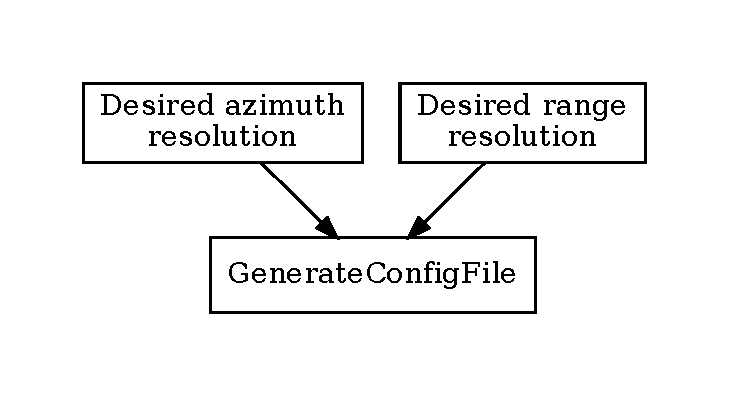
\includegraphics{sim.pdf}}
 \caption{Simulation of the SURE signal.}
 \label{fg:simflow}
 \end{center}
\end{figure}
\subsection{Generation of the raw signals}
All simulations for this paper utilize a phased array with elements of width 0.04m which are ideally spaced 0.04m apart. For instance, the phased array used for the 40cm mode is described by the XML snippet shown in listing \ref{lst:array}.
\lstset{language=XML}
\begin{lstlisting}[caption={Phased Array configuration}, label={lst:array}]
<instrument>
  <antennaArray>
    <carrierFrequency unit="Hz">9.650e9</carrierFrequency>
    <azimuthPositions unit="m">-9.980000 -9.940000 -9.900000 ...
    ... 9.900000 9.940000 9.980000</azimuthPositions>
    <azimuthElementLengths unit="m">0.040000 0.040000 0.040000 ...
    ... 0.040000 0.040000 0.040000</azimuthElementLengths>
    <transmitPowers unit="dB">10.0 10.0 10.0 ...
    ... 10.0 10.0 10.0</transmitPowers>
    <systemTemperature unit="degrees" system="Kelvin">297</systemTemperature>
    <systemLosses unit="dB">-5.3</systemLosses>
  </antennaArray>
</instrument>
\end{lstlisting}
The azimuthPositions XML field defines the position of each T/R module in the azimuth direction while the azimuthElementLength defines the width of each element.
\par
The various azimuth look directions are defined according to the angular width of each beam (which depends upon the length of the subaperture) and the span of angles required to achieve a particular azimuth resolution. In this simulation all beams are created with the same angular width. As well, the subaperture phase-centre positions are generated to be evenly spaced in the azimuth direction.
\begin{figure}[h!]
\begin{center}
 \resizebox{0.8\columnwidth}{!}{\input{subarray.pdf_tex}}
 \caption{Schematic of 5 subapertures for the 40 cm mode.}
 \label{fg:fivechansubaperture}
 \end{center}
\end{figure}
\par
As illustrated in \fgref{fg:fivechansubaperture}, the simulation generates a data array for each subaperture/beam combination. The parameters for for each subaperture/beam combination are also read from the configuration file as illustrated in listing \ref{lst:configuration}. For each of these combinations, the configuration file defines an XML element called radarConfiguration which has a channel attribute given by ``channel$m$-$n$'', where $m$ corresponds to the subaperture while $n$ corresponds to the beam. The subaperture is defined using magnitude weights for each phased-array element on both transmit and receive. The set of wieghts used on transmit may be different from those used on receive. 
\par
The beam directions is controlled using true time-delays on both transmit and receive (although they are set to the same values in this simulation so that the transmit and receive beams are pointing in the same direction). Of course, a true time-delay approach rather than a phase-steered approach is required as we are considering a wide-band system rather than a narrow-band system.
\begin{lstlisting}[caption={Channel/Beam configuration}, label={lst:configuration}]
<radarConfiguration channel="channel0-0">
  <transmitConfiguration>
    <polarization>H</polarization>
    <u0 unit="radians">1.553329e-02</u0>
    <magnitude unit="natural">0 0 0 ... 1 1 1 ... 0 0 0</magnitude>
    <truedelay unit="ns">0.517098 0.515026 0.512953 ...</truedelay>
  </transmitConfiguration>
  <receiveConfiguration>
    <polarization>H</polarization>
    <u0 unit="radians">1.553329e-02</u0>
    <magnitude unit="natural">1 1 1 ... 0 0 0 ... 0 0 0</magnitude>
    <truedelay unit="ns">0.517098 0.515026 0.512953 ...</truedelay>
  </receiveConfiguration>
</radarConfiguration>
\end{lstlisting}
A set of data for each subaperture/beam combination is created with the data stored in the undersampled azimuth-wavenumber, range-time domain. The number of samples in each of the subaperture/beam combinations is sufficient in the range direction to cover all range-cell migration and sufficient in the azimuth direction to capture all angles covered by every beam. Since the number of beams equals the number of channels, the total numer of channels created is $\numberChannels = (\channelM+1)^2$.
\par
Note that in this simulation, the computed signals have no across-track baseline.
\subsection{Multichannel processing}
Multichannel processing for this simulation occurs in the azimuth-wavenumber, range-time domain. This step computes a processing filter that attempts to create a signal over an azimuth frequency range given by $\kparmPRF*(\numberChannels + 4)$; that is, when the average antenna pattern of \eqref{eq:averagePattern} is applied, there should some wavenumber domain zero-padding applied to the computed signal.
\par
Since the theory shows that the multichannel processing filter is range independent, only a single processing filter is computed an applied across all ranges. Figure \fgref{fg:reconstructed} illustrates the multichannel processing signal. In the figure, one sees that the response in the Doppler domain shows the desired response as a function of $\kparm$, with each local maximum in this region highlighting the response from each sub-beam.
\begin{figure}[ht!]
\begin{subfigure}{0.5\textwidth}
\begin{center}
 \resizebox{\columnwidth}{!}{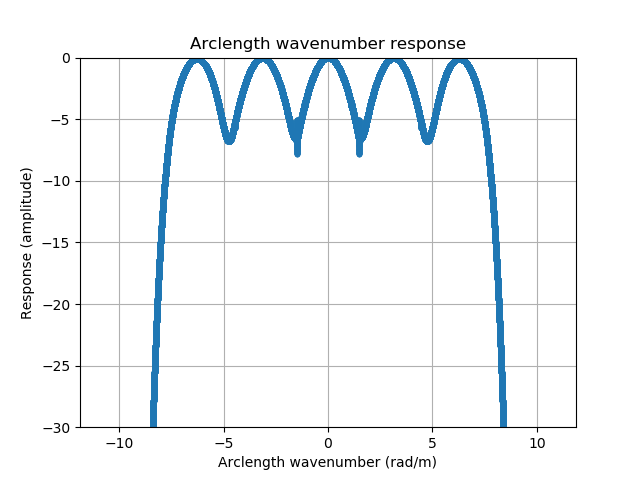
\includegraphics{simulation/40cm/simulation_plots/wk_doppler_response_amplitude.png}}
 \caption{40 cm mode.}
 \label{fg:40cmreconstructed}
 \end{center}
\end{subfigure}
\begin{subfigure}{0.5\textwidth}
\begin{center}
 \resizebox{\columnwidth}{!}{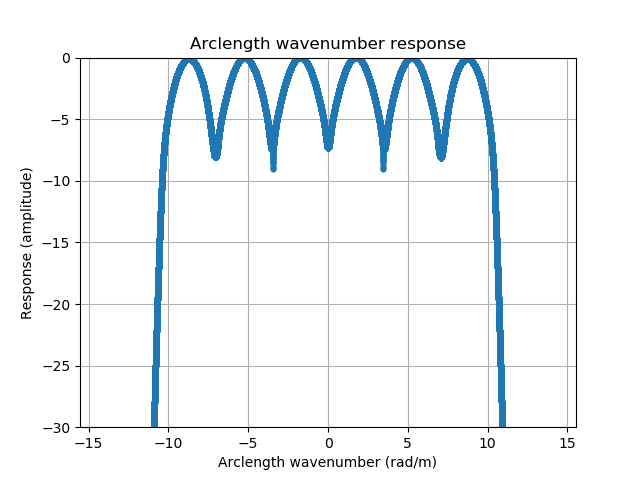
\includegraphics{simulation/30cm/simulation_plots/wk_doppler_response_amplitude.png}}
 \caption{30 cm mode.}
 \label{fg:30cmreconstructed}
 \end{center}
\end{subfigure}
\begin{subfigure}{0.5\textwidth}
\begin{center}
 \resizebox{\columnwidth}{!}{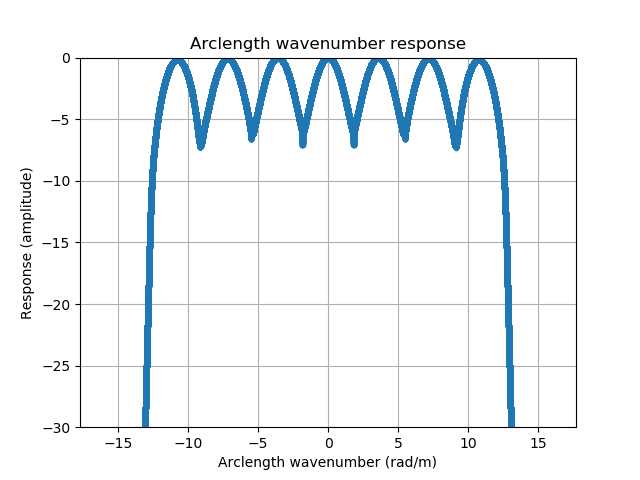
\includegraphics{simulation/25cm/simulation_plots/wk_doppler_response_amplitude.png}}
 \caption{25 cm mode.}
 \label{fg:25cmreconstructed}
 \end{center}
\end{subfigure}
\begin{subfigure}{0.5\textwidth}
\begin{center}
 \resizebox{\columnwidth}{!}{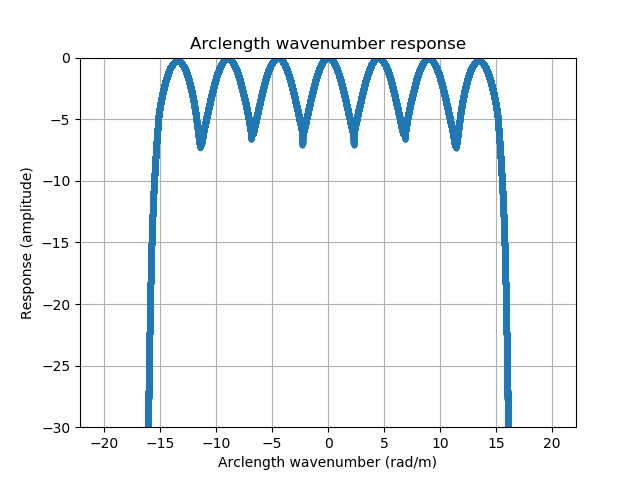
\includegraphics{simulation/20cm/simulation_plots/wk_doppler_response_amplitude.png}}
 \caption{20 cm mode.}
 \label{fg:20cmreconstructed}
 \end{center}
\end{subfigure}
\begin{subfigure}{0.5\textwidth}
\begin{center}
 \resizebox{\columnwidth}{!}{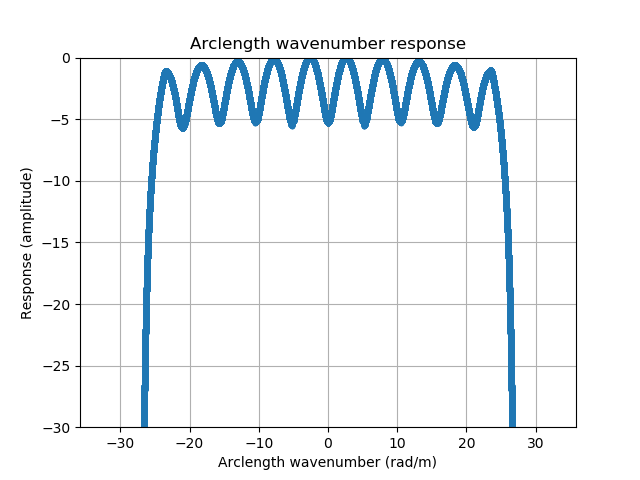
\includegraphics{simulation/12cm/simulation_plots_full/wk_doppler_response_amplitude.png}}
 \caption{12 cm mode.}
 \label{fg:12cmreconstructed}
 \end{center}
\end{subfigure}
\begin{subfigure}{0.5\textwidth}
\begin{center}
 \resizebox{\columnwidth}{!}{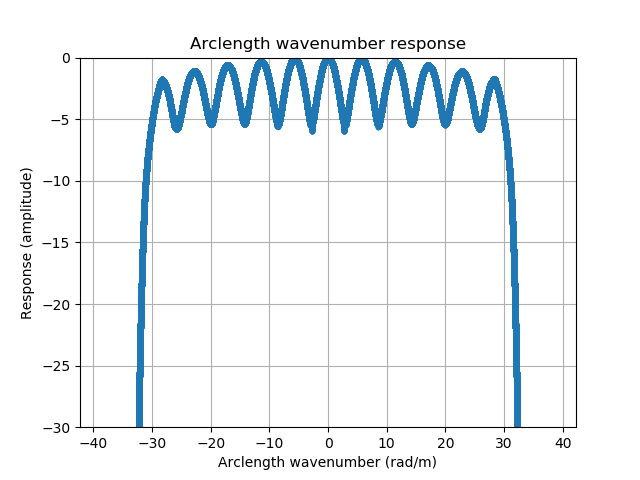
\includegraphics{simulation/10cm/simulation_plots_phase_corrected/wk_doppler_response_amplitude.png}}
 \caption{10 cm mode.}
 \label{fg:10cmreconstructed}
 \end{center}
\end{subfigure}
\caption{Reconstructed signals in azimuth wavenumber domain.}
\label{fg:reconstructed}
\end{figure}
\clearpage
\subsection{Azimuth compression}
The simulator then azimuth compresses multichannel reconstructed signal with the generalized Stolz interpolation algorithm outlined in \scref{sc:modifiedStolz}. \Fgref{fg:PSFAll} illustrates the produced the Point Spread Functions (PSF) for all modes. In these plots, the residual phase correction of \scref{sc:phaseCompensation} has not been applied.
\begin{figure}[ht!]
\begin{subfigure}{0.5\textwidth}
\begin{center}
 \resizebox{\columnwidth}{!}{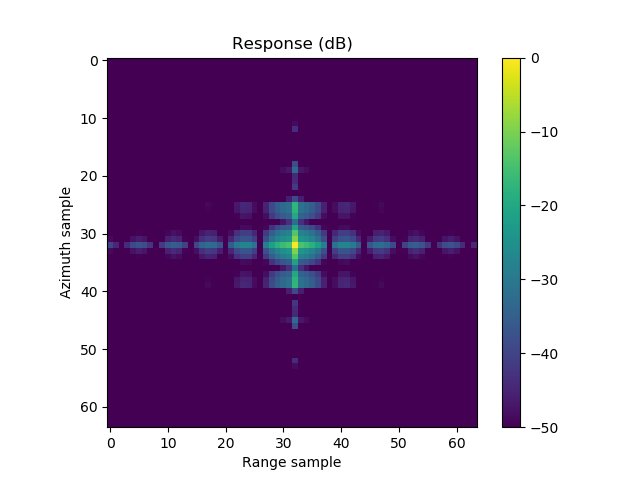
\includegraphics{simulation/40cm/simulation_plots/wk_response_32x32.png}}
 \caption{40 cm mode.}
 \label{fg:40cmPSF}
 \end{center}
\end{subfigure}
\begin{subfigure}{0.5\textwidth}
\begin{center}
 \resizebox{\columnwidth}{!}{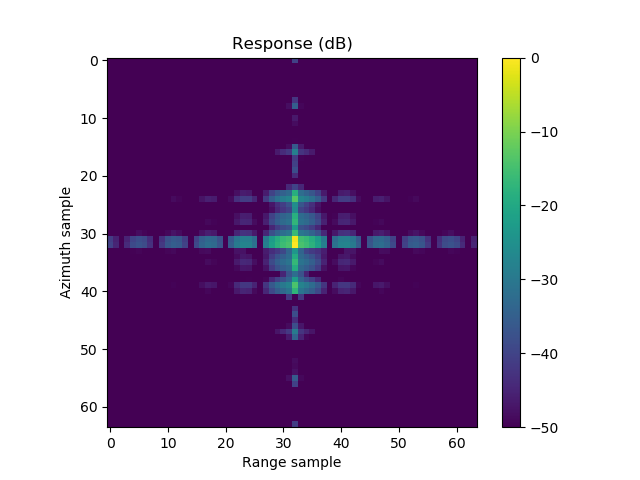
\includegraphics{simulation/30cm/simulation_plots/wk_response_32x32.png}}
 \caption{30 cm mode.}
 \label{fg:30cmPSF}
 \end{center}
\end{subfigure}
\begin{subfigure}{0.5\textwidth}
\begin{center}
 \resizebox{\columnwidth}{!}{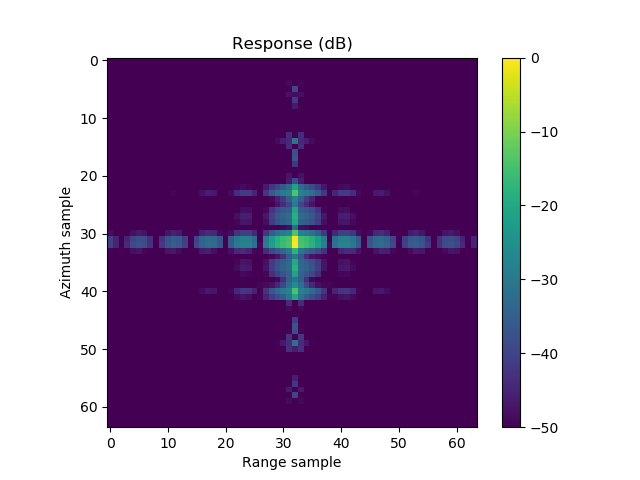
\includegraphics{simulation/25cm/simulation_plots/wk_response_32x32.png}}
 \caption{25 cm mode.}
 \label{fg:25cmPSF}
 \end{center}
\end{subfigure}
\begin{subfigure}{0.5\textwidth}
\begin{center}
 \resizebox{\columnwidth}{!}{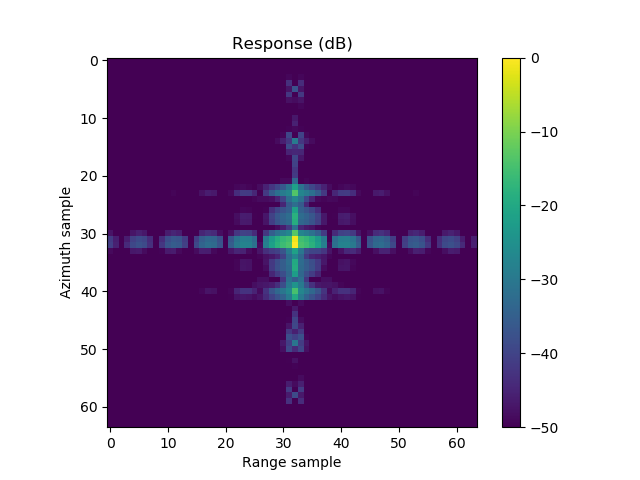
\includegraphics{simulation/20cm/simulation_plots/wk_response_32x32.png}}
 \caption{20 cm mode.}
 \label{fg:20cmPSF}
 \end{center}
\end{subfigure}
\begin{subfigure}{0.5\textwidth}
\begin{center}
 \resizebox{\columnwidth}{!}{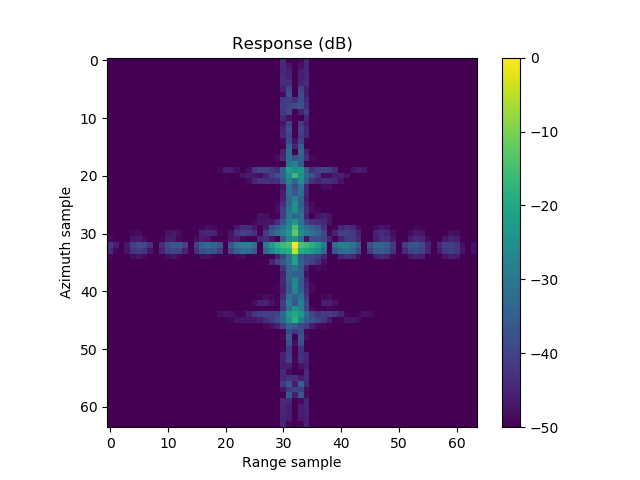
\includegraphics{simulation/12cm/simulation_plots_full/wk_response_32x32.png}}
 \caption{12 cm mode.}
 \label{fg:12cmPSF}
 \end{center}
\end{subfigure}
\begin{subfigure}{0.5\textwidth}
\begin{center}
 \resizebox{\columnwidth}{!}{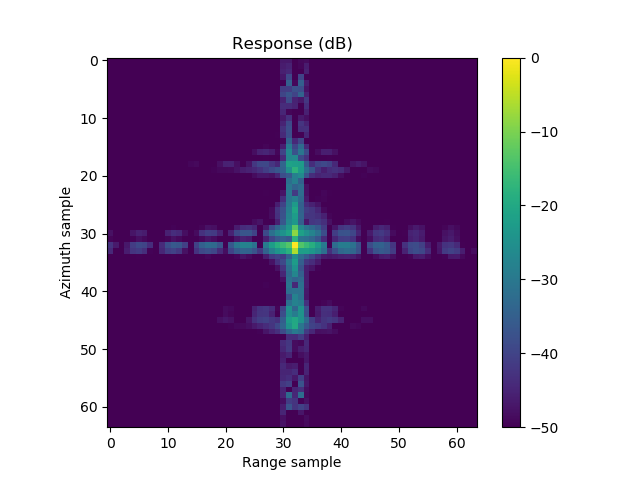
\includegraphics{simulation/10cm/simulation_plots/wk_response_32x32.png}}
 \caption{10 cm mode.}
 \label{fg:10cmPSF}
 \end{center}
\end{subfigure}
\caption{Processed signal Point Spread Response.}
\label{fg:PSFAll}
\end{figure}
\clearpage
\subsubsection{Residual phase correction}
As the resolution increases, it becomes more important to compensate for the residual phase difference that arises from the discrepancy between the differential geometry approximation to the orbit and the true satellite orbit. If exmained closely, \fgref{fg:10cmPSF} shows an azimuth imbalance in the the PSF for the 10cm mode (this can also be seen in the 12cm mode and in the 20 cm mode). This imbalance is made clearer in the cross-section plot of \fgref{fg:azimuthCross10Unbalanced}
\begin{figure}[ht!]
\begin{center}
 \resizebox{\columnwidth}{!}{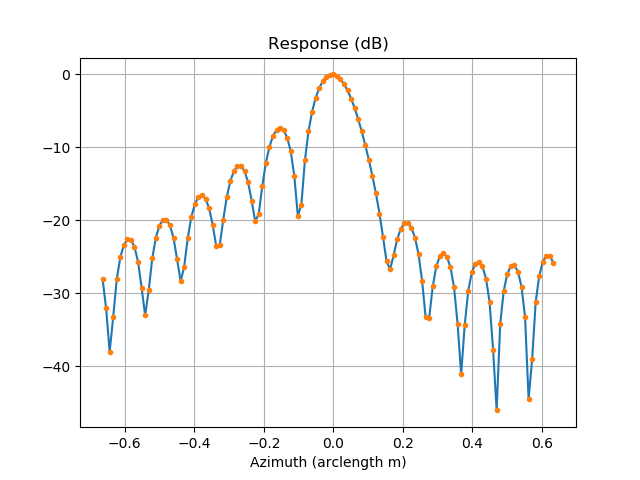
\includegraphics{simulation/10cm/simulation_plots/wk_response_s_os_8.png}}
 \caption{Azimuth cross-section of 10cm mode without residual phase correction.}
 \label{fg:azimuthCross10Unbalanced}
 \end{center}
\end{figure}
After compensating for the residual phase using the computed phase compensation described in \scref{sc:phaseCompensation}, one obtains the more desirable point spread function illustrated in \fgref{fg:10cmPSFBalanced} along with its azimuth cross-section illustrated in \fgref{fg:azimuthCross10}.
\begin{figure}[ht!]
\begin{center}
 \resizebox{\columnwidth}{!}{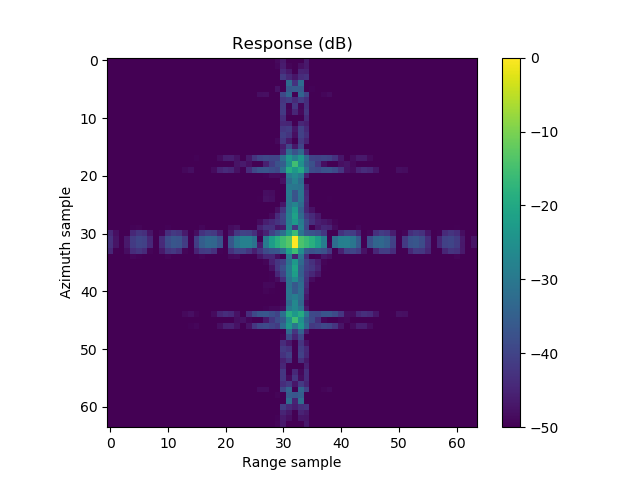
\includegraphics{simulation/10cm/simulation_plots_phase_corrected/wk_response_32x32.png}}
 \caption{Point Spread Function of 10cm mode after phase compenstaion.}
 \label{fg:10cmPSFBalanced}
 \end{center}
\end{figure}
\begin{figure}[ht!]
\begin{center}
 \resizebox{\columnwidth}{!}{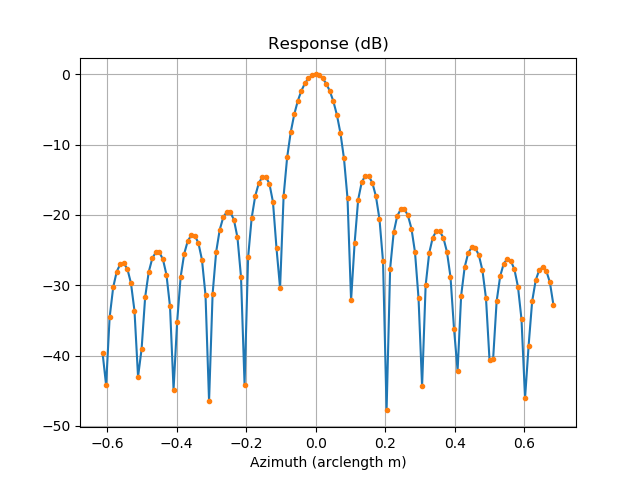
\includegraphics{simulation/10cm/simulation_plots_phase_corrected/wk_response_s_os_8.png}}
 \caption{Azimuth cross-section of 10cm mode after residual phase correction.}
 \label{fg:azimuthCross10}
 \end{center}
\end{figure}
The plot clearly illustrates a 3dB resolution of better than 10cm. Further, in the generation of sidelobes at this zoom level, the peak sidelobe level is at around -14.5dB from the peak.
\par
Over the wider range of azimuth values illustrated in \fgref{fg:azimuthCross10wide}, one observes a different generation of sidelobes. The peak of these second-level sidelobes manifests at around -18dB. A suitable weighting on the Doppler response of \fgref{fg:10cmPSF} can suppress these second-level sidelobes at the expense of resolution.
\begin{figure}[ht!]
\begin{center}
 \resizebox{\columnwidth}{!}{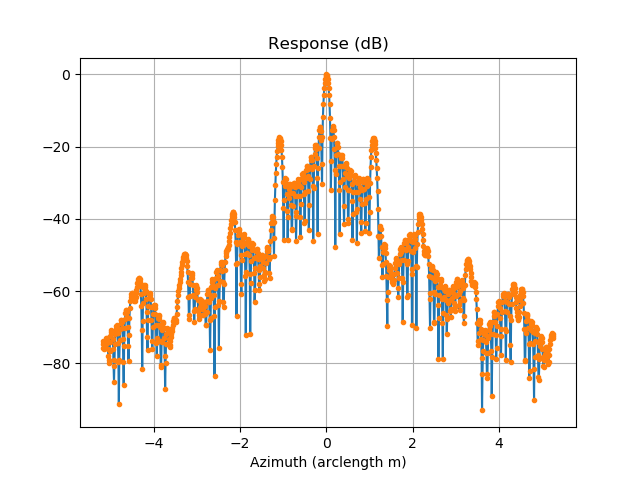
\includegraphics{simulation/10cm/simulation_plots_phase_corrected/wk_response_s_os_64.png}}
 \caption{Azimuth cross-section of 10cm mode after residual phase correction.}
 \label{fg:azimuthCross10wide}
 \end{center}
\end{figure}
% shown in \fgref{fg:psf}. This figure illustrates that the system achieves the desired resolution with the response width less than 0.1 m at the -5 dB level. While the figure also shows a second set of sidelobes at -15 dB, it is assumed that these can be reduced by an appropriate choice of weighting on the antenna patterns. 
% \begin{figure}[ht!]
% \begin{center}
%  \resizebox{\columnwidth}{!}{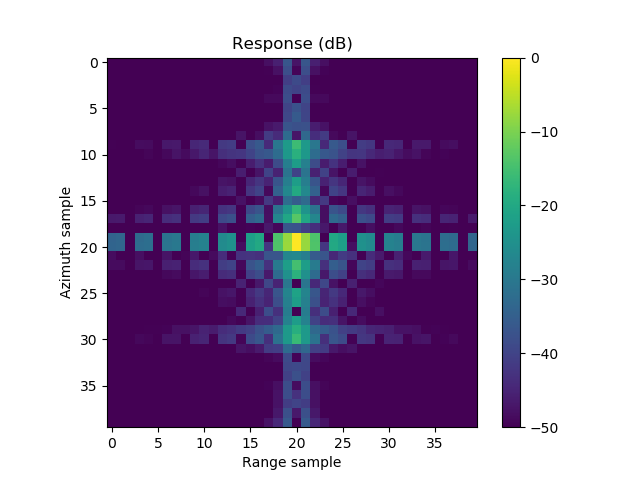
\includegraphics{simulation/Figure_11.png}}
%  \caption{Point Spread Function using the described processing method.}
%  \label{fg:psf}
%  \end{center}
% \end{figure}
% \begin{figure}[ht!]
% \begin{center}
%  \resizebox{\columnwidth}{!}{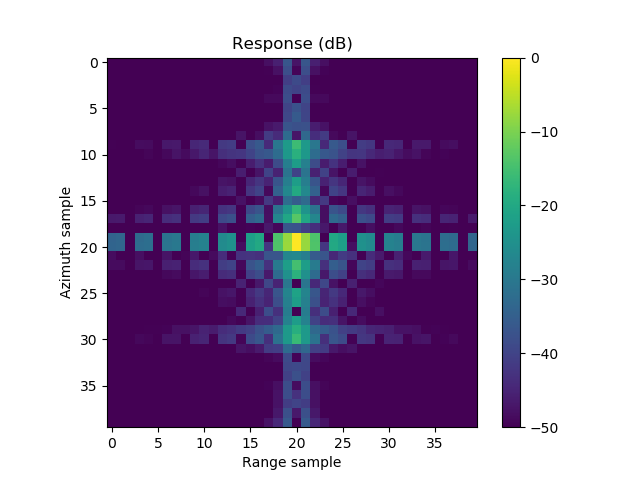
\includegraphics{simulation/Figure_11.png}}
%  \caption{Point Spread Function using the described processing method.}
%  \label{fg:psf1}
%  \end{center}
% \end{figure}
% \begin{figure}[ht!]
% \begin{center}
%  \resizebox{\columnwidth}{!}{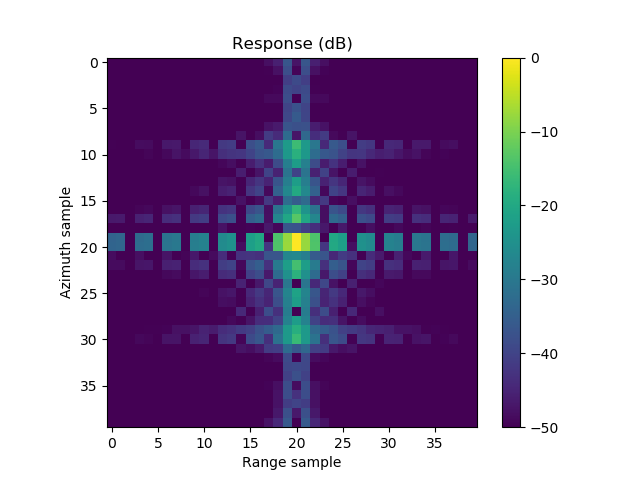
\includegraphics{simulation/Figure_11.png}}
%  \caption{Point Spread Function using the described processing method.}
%  \label{fg:psf2}
%  \end{center}
% \end{figure}
\subsubsection{Sigal to noise ratio}
The PRFs selected for all simulations differ from the ``ideal'' PRF thus potentially adversely affecting the Signal to Noise Ratio (SNR). As a measure of the radiometrical resolution, the Noise Equaivalent Sigma Zero (NESZ) is computed for all modes. 
Based upon parameters in the simulation configuration file, the radar equation is used to generate a estimate of the simulated signal to noise ratio. 
\begin{equation}
 \frac{P_{av}\lambda_0}{(4\pi)^3r^4Lk_BT}
\end{equation}

A test noise signal is also generated by the simulator. The SNR prior to filtering is compared with the SNR after filtering (but before azimuth compression) giving a change of about -0.4 dB. This shows that with the simulated parameters, the SNR does not change significantly.
\begin{table}[ht!]
\begin{center}
 \caption{Computed NESZ}
 \label{tb:nesz}
 \begin{tabular}{r|l|l}
 {\bf Mode} & {\bf $f_p$} (Hz)& {\bf NESZ} (dB)\\\hline
 {\bf 40 cm} & 4500.00 & -30.9\\\hline
 {\bf 30 cm} & 5000.00 & -29.8\\\hline
 {\bf 25 cm} & 5142.86 & -29.7\\\hline
 {\bf 20 cm} & 6428.57 & -29.2\\\hline
 \end{tabular}
 \end{center}
\end{table}
\par
In summary, the simulation demonstrates the suitability of the proposed signal processing algorithm and also shows how the generated PSF contains extra sidelobes that most likely result from the different shape of the signal response in the Doppler domain. If these sidelobes are intolerable, they can possibly be removed by modifying the phased-array beam tables; however, this is a topic for further research.
\clearpage
%\section{Conclusion}
We propose a system for improved space-based SAR imaging, describing the design, which is based upon a phased-array and an appropriate switching network to allow digitisation of multiple receive channels, the configuration, which imposes a rapid electronic beam switching capability upon the design, and a suitable signal processing algorithm to compute the high resolution imagery. The proposed configuration permits measurement of a relatively large swath in a Stripmap-like mode, thereby offering, theoretically, unlimited azimuth extent. On the other hand, as demonstrated by the test example of 10cm azimuth resolution considered throughout the paper, the resolution of the imagery can be even better than the highest resolution spotlight imagery available from current commercial systems.
\par
Importantly, the state of current technology is sufficiently advanced to construct such a SAR system.
\par
As a final important consideration, we note that the design does not preclude the use of other traditional measurement modes such as Spotlight, TOPS or ScanSAR. Further, it provides the flexibility to implement other advanced modes such as HRWS and Ground Moving Target Indication.

